\section{Working hours}

This attack aims to gather as much information about the working hour behaviour as possible.
Information which can be extracted by this attack is for example the sleep rhythm of the target.
It can be used to detect whether the target is a person working regular shifts from from Monday to Friday or rather a freelancer or open-source contributor working at the weekend.
The attack can be further used to compare the working hour patterns of several people in the same project or organization.
For instance this could be used to infer relationships between colleagues, based on an equal working shift.

\subsection{Implementation}

\begin{figure}[H]
    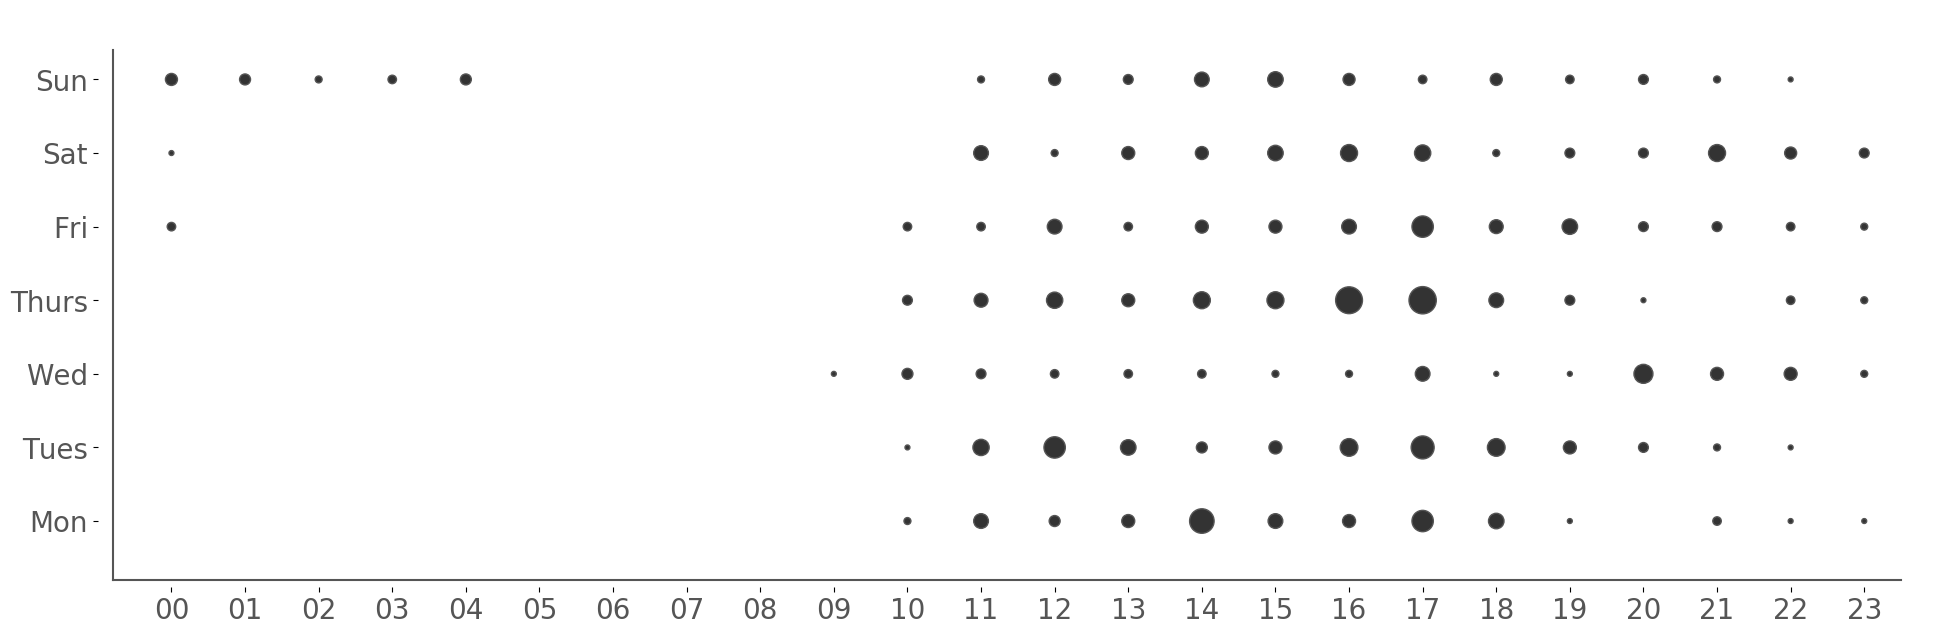
\includegraphics[scale=0.20]{./graphs/analysis/ordered-punchcard}
    \centering
    \caption{Punchcard of the sleep rhythm analysis of the author.}\label{fig:working-hour-rhythm-author}
\end{figure}

\begin{figure}[H]
    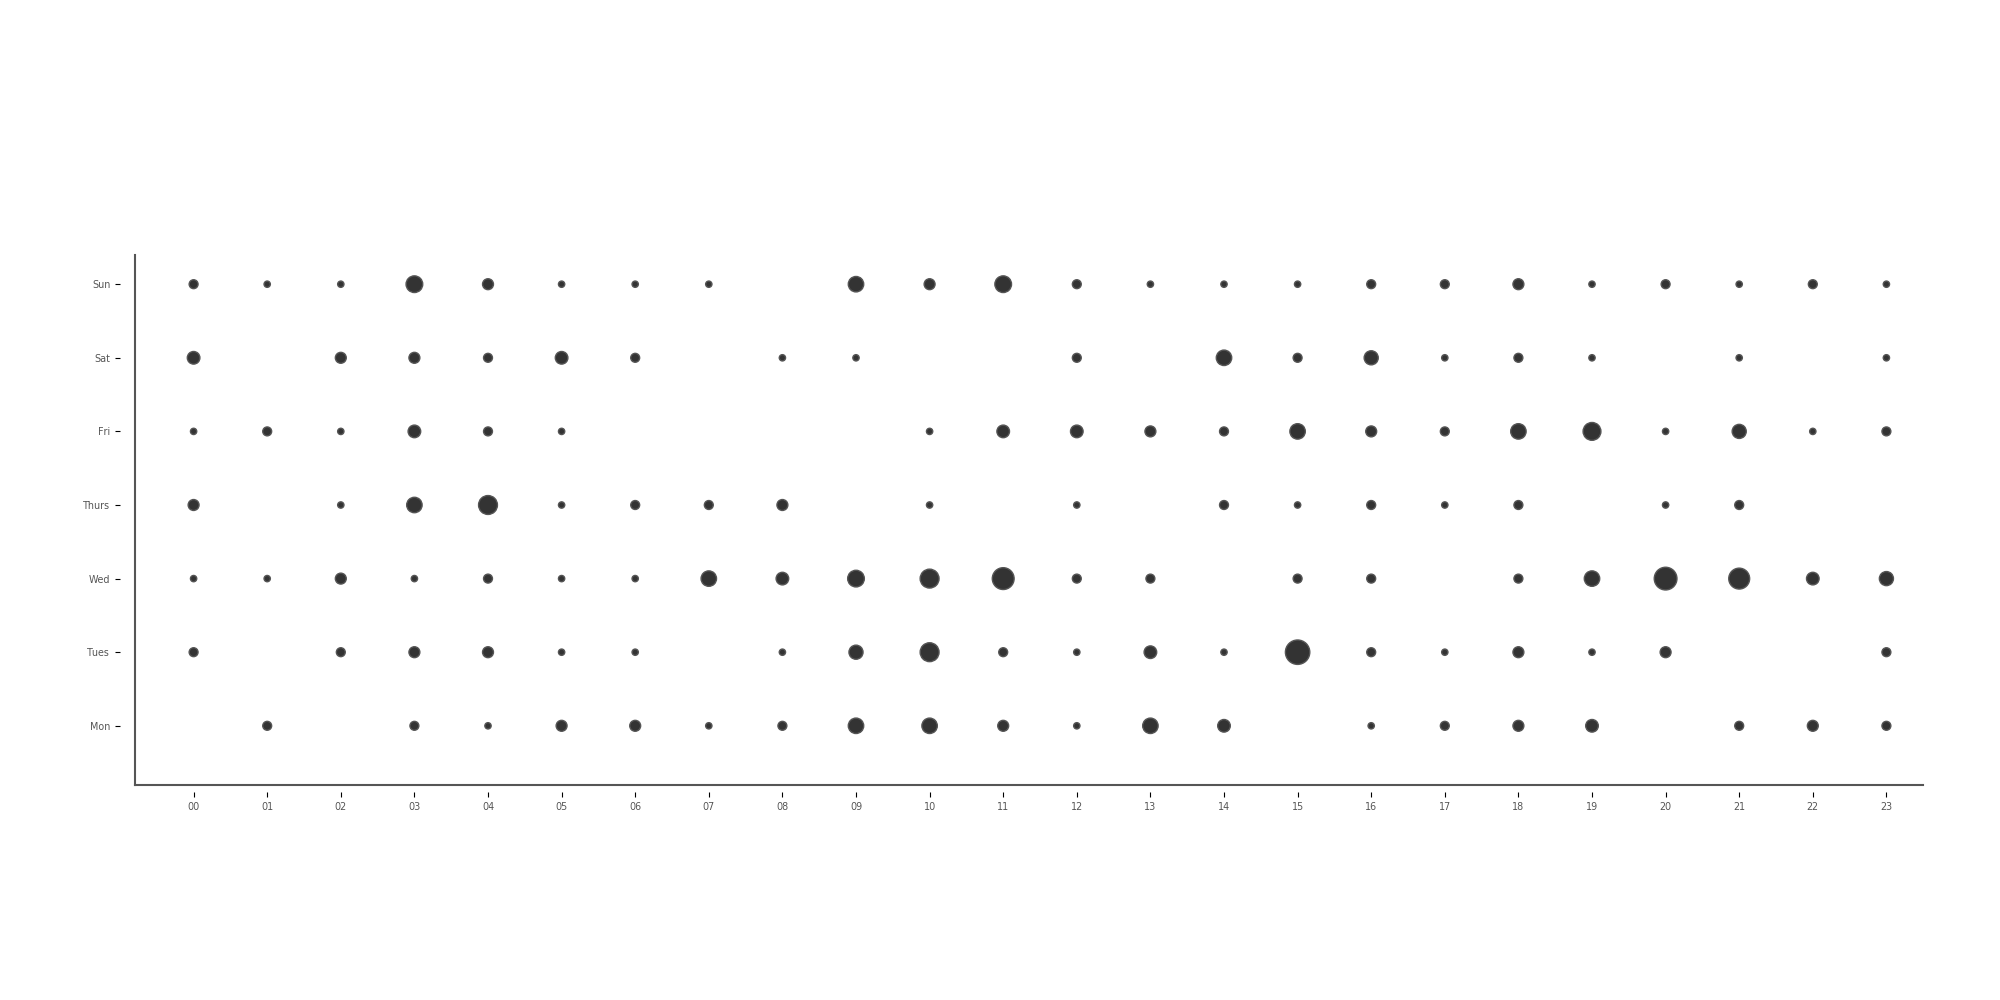
\includegraphics[scale=0.20]{./graphs/analysis/random-punchcard}
    \centering
    \caption{Punchcard of an user without a regular sleep rhythm.}\label{fig:random-sleep-rhythm}
\end{figure}

\begin{figure}[H]
    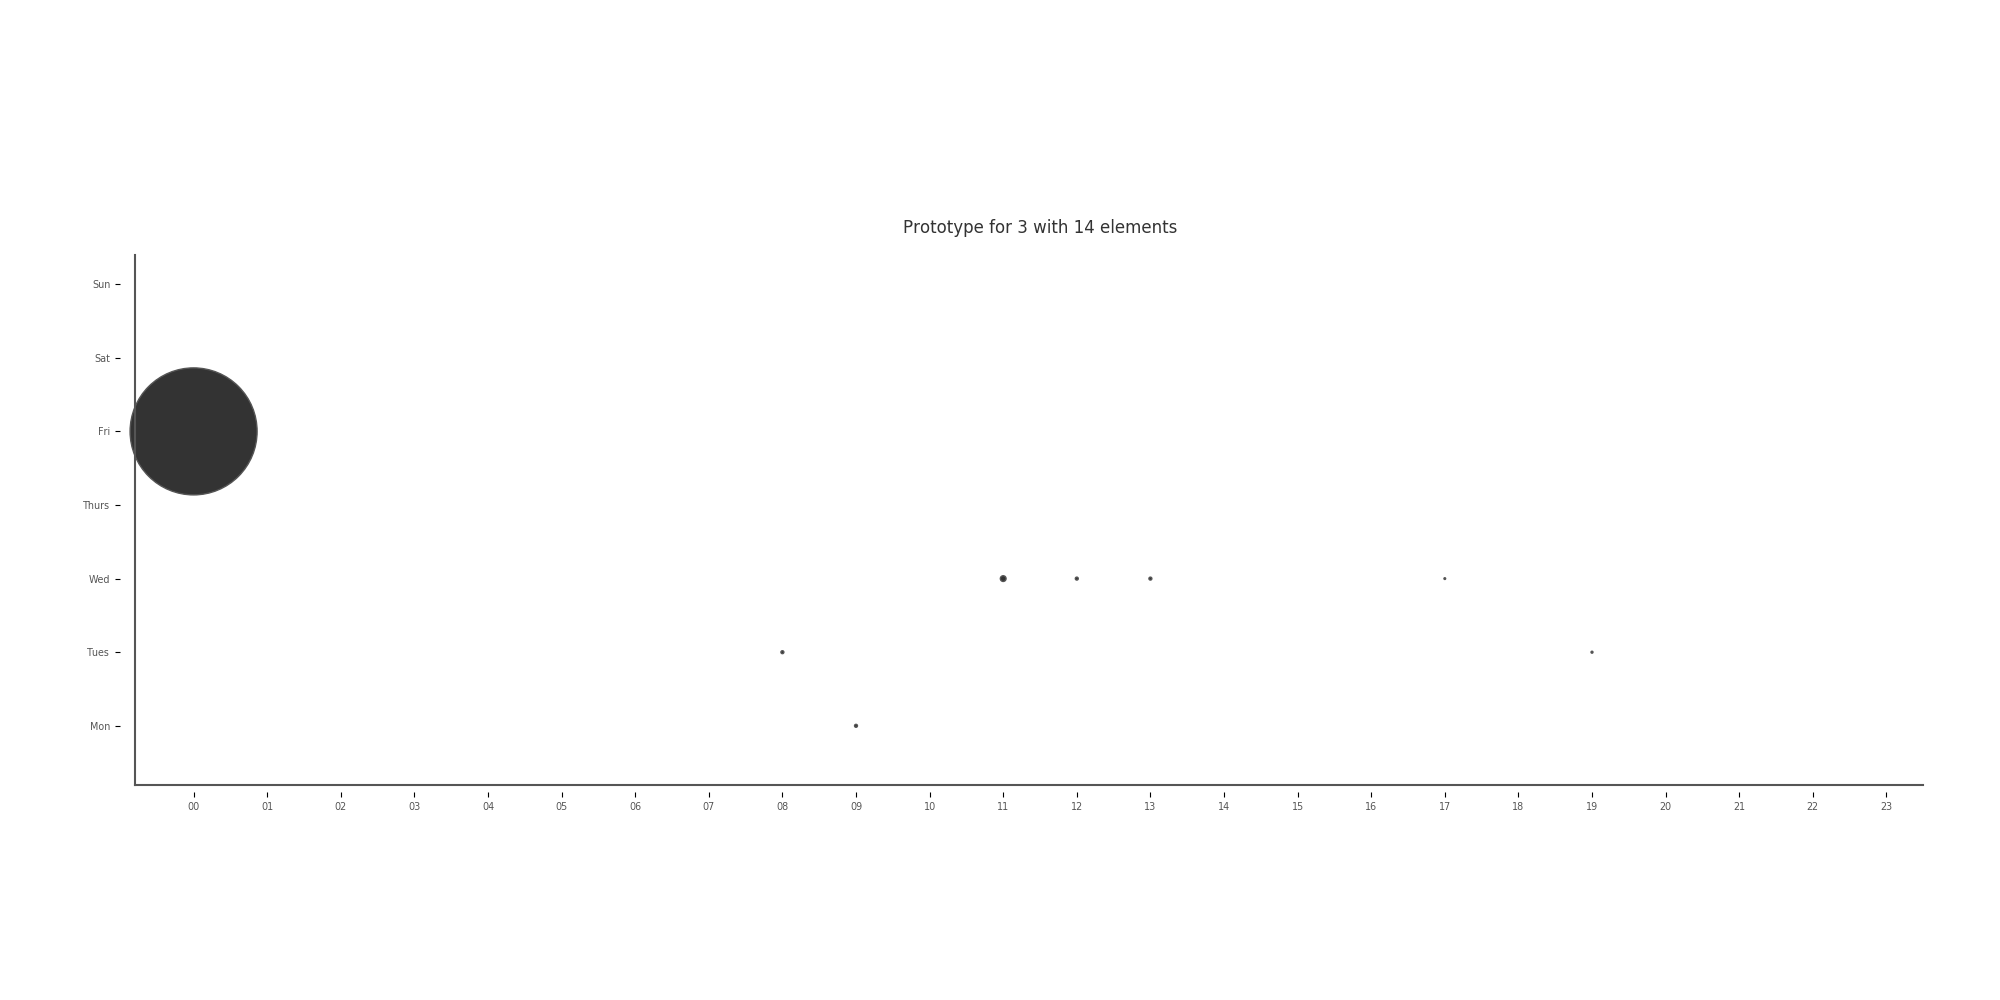
\includegraphics[scale=0.20]{./graphs/analysis-affinity/3}
    \centering
    \caption{The work time analysis of the author.}\label{fig:missing-time}
\end{figure}
